\documentclass[hidelinks, 10pt,a4paper]{article}

\usepackage[english,francais]{babel}
\usepackage[utf8]{inputenc}
\usepackage{geometry}
\usepackage[T1]{fontenc}
\usepackage[pdftex]{graphicx}
\usepackage{adjustbox}
\usepackage{color}
\usepackage{setspace}
\usepackage{hyperref}
\usepackage[french]{varioref}
\usepackage{comment}
\usepackage{pgfgantt}


\usepackage{fancyhdr}
\pagestyle{fancy}

\renewcommand{\headrulewidth}{1pt}
\fancyhead[L]{}
\fancyhead[C]{\textbf{UML Reverse}}
\fancyhead[R]{
\includegraphics[width=2cm]{imgPDD/universite-rouen.jpg}}

\title{\bfseries Plan de développement\\Projet UML Reverse}
\geometry{hmargin=2.5cm,vmargin=3cm}

\begin{document}
\maketitle
\begin{center}
\begin{tabular}{ll}
  Version~: & 1.0\\[.5em]
  Date~: & \date{\today}\\[.5em]
  Rédigé par~: & Florian \textsc{Inchingolo}\\
               & Anthony \textsc{Godin}\\
               &\\[.5em]
  Relu par~:   & Florian \textsc{Inchingolo}\\
               & Anthony \textsc{Godin}\\
               &\\
\end{tabular}
\end{center}

\newpage
\begin{center}
    \section*{Mises à jour}
    \begin{tabular}{|c|c|p{8cm}|}
        \hline{\textbf{Version}} & {\textbf{Date}} & {\textbf{Modifications réalisées}}\\\hline
        {1.1} & {29/01/2016} & {Rectification du Gantt, des itérations et de l'implémentation du Scrum}\\\hline
        {1.0} & {21/01/2016} & {Corrections avant la présentation}\\\hline
        {0.1} & {10/01/2016} & {Début de la rédaction du PDD}\\\hline
    \end{tabular}
\end{center}

\newpage
\tableofcontents

\newpage
\section{Contexte du projet}
\subsection{Fiche du projet}
Dans le cadre de la formation de première année en Master en Génie Informatique Logiciel (GIL)
de l'UFR de Sciences et Techniques de Rouen, un projet annuel en équipe de 6 ou 7 personnes
est proposé parmi une liste imposée.

\subsubsection*{Vision}
Le but du projet est d'obtenir un éditeur de diagrammes UML2. Ce diagramme pourra
être obtenu à partir d'un fichier PlantUML, à partir d'un ensemble de sources Java
ou être créé de toutes pièces via l'éditeur. Chaque entité du diagramme doit pouvoir
être déplacée ou stylisée.

\subsubsection*{Objectifs}
L'application devra :
\begin{itemize}
\item être modulaire et documentée ;
\item être ergonomique ;
\item respecter UML2.
\end{itemize}

\subsubsection{Matrice des leviers}

\begin{center}
\begin{tabular}{|r|c|c|c|}
   \hline{} & {\textbf{Souple}} & {\textbf{Moyen}} & {\textbf{Rigide}} \\\hline
   {\textbf{Coût / Temps}} & {X} & {} & {} \\\hline
   {\textbf{Durée}} & {} & {} & {X} \\\hline
   {\textbf{Qualité}} & {} & {} & {X} \\\hline
   {\textbf{Portée}} & {} & {X} & {} \\\hline
\end{tabular}
\end{center}

\subsection{Phases de développement}
Ce projet se déroule en deux phases imposées. La première,
la \textbf{phase d'analyse}, est la conception des documents nécessaires pour
mener le projet à bien. Cette phase se rapproche des méthodes de développement
classiques. La deuxième phase est la \textbf{phase de développement}, qui consiste
à développer l'application issue des besoins et des documents définis lors de la
phase d'analyse. Cette phase doit se dérouler en utilisant des méthodes de développement
agiles pour s'assurer de rendre un projet dans les temps en respectant le plus possible 
les attentes du client.

\newpage
\section{Terminologie}
  Se référer au document terminologie.

\section{Préparation du projet}
\subsection{Organisation de l'équipe}
Nous avons défini au début de projet plusieurs rôles, que nous avons affiné au
fur et à mesure de la conception du projet :
\begin{tabular}{ll}
{Anthony \textsc{Godin}} & {Chef de projet et Responsable client} \\
{Florian \textsc{Inchingolo}} & {Responsable de l'architecture du parseur} \\
{Yohann \textsc{Henry}} & {Responsable de l'architecture du modèle} \\
{Nabil \textsc{Belkhous}} & {Responsable des tests} \\
{Nicolas \textsc{Meniel}} & {Développeur} \\
{Stephen \textsc{Cauchois}} & {Responsable de l'architecture graphique} \\
{Saad \textsc{M'Rabet}} & {Développeur} \\
\end{tabular}

A noter, chaque membre de l'équipe du projet est aussi bien entendu développeur.

\subsection{Scrum}
  Nous avons choisi d'utiliser une méthode de développement agile et plus particulièrement Scrum 
  pour répondre le mieux possible au besoin du client en ``l'intégrant`` dans notre équipe.
  Grâce à cette méthode nous pourrons régulièrement faire intervenir notre client pour modéliser
  le produit de la façon la plus proche possible de l'envie du client.
  
  C'est pourquoi nous avons prévu 3 itérations qui composeront ensembles le projet.
  Au début de chaque itération, nous ferons une \emph{préparation de Sprint} afin de planifier
  les tâches nécessaires ainsi que de les répartir. Nous utiliserons un \emph{Sprint Backlog}
  afin d'aider à la préparation du sprint.
  Le développement pourra ensuite commencer.
  Celui-ci sera dirigé par les tests qui seront écrits après le développement
  de chaque classe. Les tests unitaires seront effectués par le développeur.
  
  Une mélée de 30 minutes sera organisée une fois par semaine (le lundi à 10h) afin que toute
  l'équipe soit au courant de l'avancement de chacun, et ainsi déterminer une possible surcharge
  de travail de chacun, ou de préciser les tâches prévues par chacun lors de ce rendez-vous.
  Des rendez-vous ponctuels de développement sont également prévu (un rendez-vous juste après la mélée hebdomadaire et un le jeudi à 14h).
  
  Plusieurs livrables sont prévus afin de faire valider le travail par le client pendant le développement. Des réunions avec
  lui seront réalisées toutes les deux semaines pour généralement présenter un livrable. Le but est de lui faire
  tester l'application en cours afin d'avoir un avis sur les corrections à apporter avant la fin de l'itération.
  Bien sûr un livrable est prévu à la fin de chaque itération pour que le client valide le travail et passer à l'étape suivante.
  
  Une phase de test sera prévu à la fin de chaque sprint pour vérifier les tests fonctionnels
  du CDR afin de valider toutes les exigences du client.
  Chaque développeur teste les fonctionnalités et l'intégration d'une partie qu'il n'a pas contribué, afin de
  déterminer les possibles erreurs plus simplement (un regard "externe" sera mieux à même
  de trouver les problèmes fonctionnels). 
  
  Cette phase sera terminée par un \emph{Sprint Review}
  afin de vérifier l'avancement concret du projet dans son ensemble, puis d'un \emph{Sprint Rétrospective}
  pour identifier les possibles difficultés et d'identifier les points forts et faibles de l'équipe
  lors de cette itération.

\subsection{Outils utilisés}
Nous utilisons Git afin de pouvoir gérer les contributions de chacun correctement.
Chaque tâche et sous-tâche est affiché au sein de Trello, un bloc-notes collaboratif.
Tous les membres de l'équipe peuvent ainsi voir l'avancement de chacun, s'attribuer
des tâches, ou aider les autres quand ceux-ci ont trop de tâches qui leur sont
attribuées. Pour la communication au sein de l'équipe, nous utilisons Slack.

\subsection{Recherche de minimisation des risques}
Lors de l'analyse des risques, nous avons mis à jour plusieurs risques qui pouvaient
être problématiques. Pour éviter que ceux-ci puissent nuire au projet, nous avons
fait des recherches afin de maîtriser les questions n'ayant pas encore de réponse.

Par exemple, pour l'analyse lexicale du langage Java, nous utilisons Antlr, mais
personne ne maîtrisait le lexeur. Nous avons donc codé une preuve de concept en amont
de la phase de développement montrant qu'il est facilement possible d'analyser
un code source Java pour en afficher l'arbre syntaxique.

Un deuxième risque était l'utilisation de JavaFX. Même si l'un d'entre nous avait
déjà utilisé cette technologie, nous n'étions pas tous familiers avec celle-ci.
Nous avons donc décidé de créer un programme d'exemple, afin de voir les possibilités
de l'API.

Pour ce qui est de la gestion du glisser-déposer, nous avons trouvé et analysé
un programme d'exemple afin de ne pas avoir de mauvaise surprise lors du développement.

Enfin, pour les relations, nous avons défini un système à base de points afin d'amoindrir
grandement la complexité de programmation de ces dernières.

\section{Planification du projet}
Pour ce projet, nous avons estimé qu'il était bénéfique de proposer 3 livrables.
Nous comptons présenter une première version contenant seulement
ce qui est nécessaire à un début d'édition du diagramme de classes, afin de
s'atteler à tous les risques possibles de blocage dès le début. Ensuite, nous proposerons
au client notre vision de l'interface graphique pour le deuxième livrable. Nous avons prévu peu
de tâches lors de la troisième itération (diagramme de cas d'utilisation) afin de pouvoir
apporter les corrections demandées par le client sur l'IHM s'il y en a, de s'assurer que
l'on peut s'engager sur ce que l'on propose, ou dans le cas où le projet se déroule mieux
que prévu, de pouvoir préparer de nouvelles fonctionnalités.

\begin{comment}
\subsection{Les itérations}
  \begin{itemize}
    \item \textbf{Livrable 1} : Disponible à la fin de la semaine 9, ce livrable sera la
      base de notre projet. Celui-ci comprendra une partie des fonctionnalités essentielles
      à un éditeur, ainsi qu'un modèle correspondant à la version finale du projet.
      Le temps de développement nécessaire à ce livrable a été estimé entre 115 à 145 heures.
    \item \textbf{Livrable 2} : Disponible à la fin de la semaine 14, le but de ce livrable
      sera d'implémenter l'interface homme-machine la plus fidèle à l'interface attendue à
      la fin du projet.
      Le temps de développement nécessaire à ce livrable a été estimé à environ 130 heures.
    \item \textbf{Livrable 3} : Disponible à la date limite du rendu de projet (semaine 18),
      l'objet de ce livrable sera l'ajout du diagramme de cas d'utilisation, et si possible, des
      fonctionnalités supplémentaires.
      Le temps de développement nécessaire à ce livrable a été estimé à environ 110 heures.
  \end{itemize}
\end{comment}

\newpage
\subsection{Diagramme de Gantt}
\begin{center}
  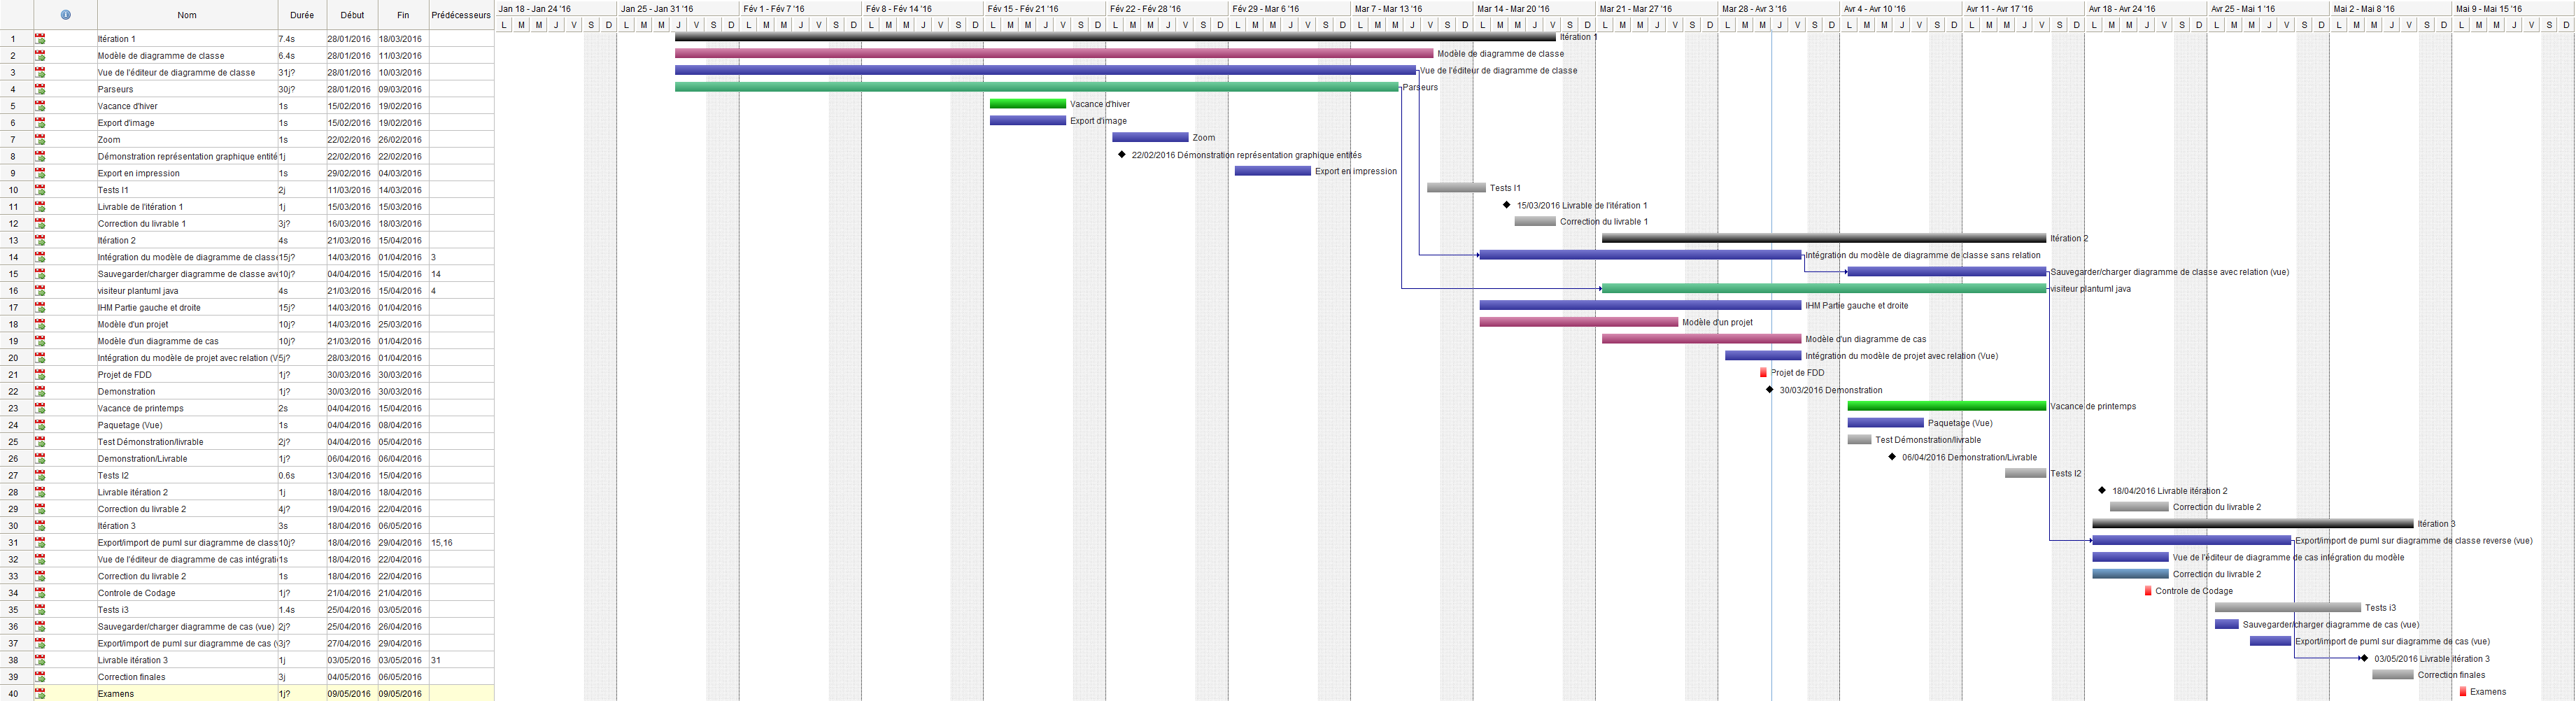
\includegraphics[angle=90,height=23cm]{imgPDD/gantt.png}
  \textit{Diagramme de Gantt}
\end{center}
\newpage
 
\begin{comment}
\begin{center}
\begin{ganttchart}{1}{14}
  \gantttitle{Numéros de semaines}{14} \\
  \gantttitlelist{5,...,18}{1} \\
  \ganttgroup{Itération 1}{1}{5} \\
  \ganttgroup{Itération 2}{6}{10} \\
  \ganttgroup{Itération 3}{11}{14} \ganttnewline[thick]
  \ganttbar{Phases de test}{5}{5}\ganttbar{}{10}{10}\ganttbar{}{14}{14} \\
  \ganttbar{Préparation du sprint}{6}{6}\ganttbar{}{11}{11} \\
  \ganttmilestone{Livrable 1}{5} \\
  \ganttmilestone{Livrable 2}{10} \\
  \ganttmilestone{Application finale}{14} \ganttnewline[thick]
  \ganttbar{Entrée / Sortie}{1}{3} \\
  \ganttbar{Modèle des diagrammes}{1}{3} \\
  \ganttbar{IHM diagramme de classes}{1}{3} \\
  \ganttbar{Déplacement des entités}{2}{3} \\
  \ganttbar{Gestion des relations}{2}{3} \ganttnewline[thick]
  \ganttbar{Finalisation de la partie centrale de l'IHM}{7}{7} \\
  \ganttbar{Partie gauche de l'IHM}{7}{9} \\
  \ganttbar{Partie droite de l'IHM}{7}{9} \\
  \ganttbar{Fonctionnalités du menu de l'application}{8}{9} \ganttnewline[thick]
  \ganttbar{IHM diagramme de cas d'utilisation}{11}{12} \\
  \ganttbar{Corrections sur l'IHM}{11}{12} \\
  \ganttbar{Finalisation du projet}{13}{14}
\end{ganttchart}
\end{center}
\end{comment}


\subsection{Itération 1}
\begin{center}
  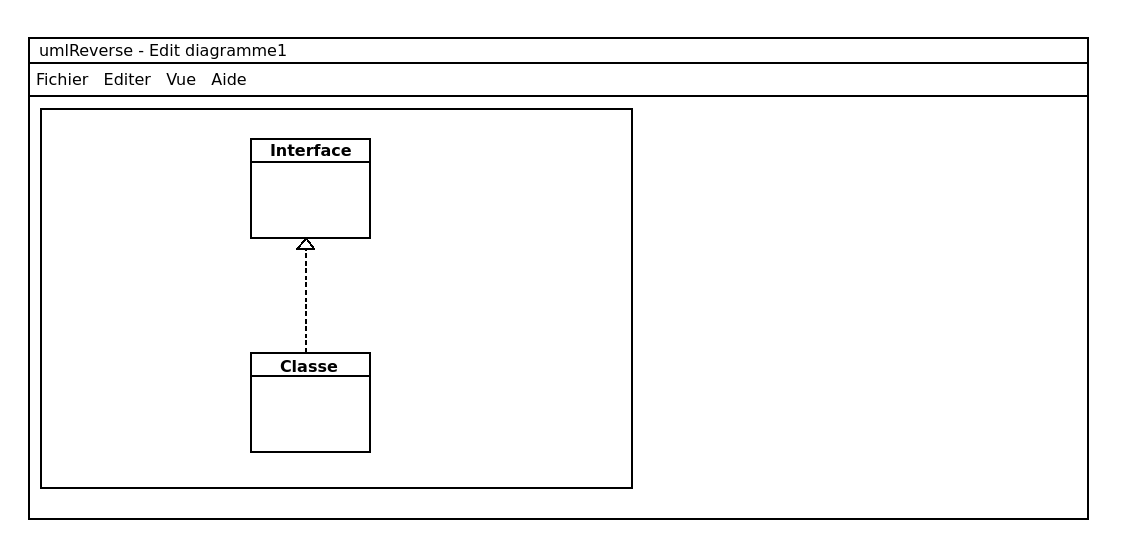
\includegraphics[width=\textwidth]{imgPDD/ihm_it1.png}
\textit{Maquette de l'interface homme-machine de l'itération 1.}
\end{center}

Disponible à la fin de la semaine 9, ce livrable sera la base de notre projet. 
Celui-ci comprendra une partie des fonctionnalités essentielles à un éditeur, ainsi 
qu'un modèle correspondant à la version finale du projet.
Le temps de développement nécessaire à ce livrable a été estimé entre 115 à 145 heures.
Le but de cette itération est de produire un premier livrable comprenant les fonctionnalités
minimales permettant d'utiliser l'application. Ce livrable permettra d'éditer totalement un diagramme de classe
(modification, exports en image et en impression, reverse etc..)
Ceci nous fait faire les tâches les plus risquées dès le début, afin de minimiser
l'impact d'autres évènements attendus ou non (comme les phases de projets ou la possibilité de la perte
d'un membre de l'équipe) sur les prochaines itérations, ainsi que d'éviter un "blocage" lors des itérations
suivantes.

\subsubsection{Fonctionnalités disponibles sur ce livrable}
\begin{itemize}
\item \textbf{IHM\_40 - IHM\_80 - IHM\_90} : Manipuler totalement un diagramme de classe
\item \textbf{MOD\_*} : Editer un diagramme de classe
 \item \textbf{CLA\_*} : Editer un diagramme de classe
\end{itemize}

\subsubsection{Définition des tâches}
\begin{itemize}
\item \textbf{Entrée / Sortie} : Création des parseurs permettant de créer un diagramme de classes à partir d'un
code Java, un diagramme compatible à partir d'un fichier PlantUML, ainsi que de charger un fichier de style à appliquer sur le diagramme.
En parallèle, création des visiteurs responsables de la sauvegarde et des exports.
\item \textbf{Modèle du diagramme de classe} : Écriture du modèle complet du diagramme de classe, comprenant le code commun
à tous les diagrammes ainsi que les classes spécifiques au diagramme de classes.
\item \textbf{Entité du modèle} : Un développeur s'occupe de coder les entités du modèle.
\item \textbf{Element du modèle} : Un développeur s'occupe de coder les éléments du modèle. 
\item \textbf{Relation du modèle} : Un développeur s'occupe de coder les relations du modèle.
\item \textbf{Regroupement et test du modèle} : Phase de tests sur le modèle.
\item \textbf{Editeur de diagramme de classe} : Développement du composant permettant l'édition du diagramme de classes
\item \textbf{D\&D des entités graphique} : Gestion du glisser-déposer sur une entité quelconque dans le composant du diagramme.
\item \textbf{Représentation graphique des entités} : Les entités sont toutes représentables graphiquement et peuvent être déplacée.
\item \textbf{Représentation graphique des relation} : Développement de l'affichage et le déplacement de toutes les relations 
      disponibles sur les diagrammes prévus.
\item \textbf{Intégrer le menu et les contrôleurs de l'application} : Assembler toutes les fonctionnalités codées dans le menu de l'application
\end{itemize}

\subsubsection{Attribution des tâches}
\begin{itemize}
\item \textbf{Entrée / Sortie} : Florian \textsc{Inchingolo}
\item \textbf{Modèle des diagrammes} : Yohann \textsc{Henry} (responsable), Nicolas \textsc{Meniel},
Nabil \textsc{Belkhous} et Saad \textsc{M'Rabet}
\item \textbf{IHM diagramme de classe} : Stephen \textsc{Cauchois} (responsable) et Anthony \textsc{Godin},
\item \textbf{Déplacement des entités} : Stephen \textsc{Cauchois}
\item \textbf{Gestion des relations} : Anthony \textsc{Godin}
\end{itemize}

\subsection{Itération 2}
\begin{center}
  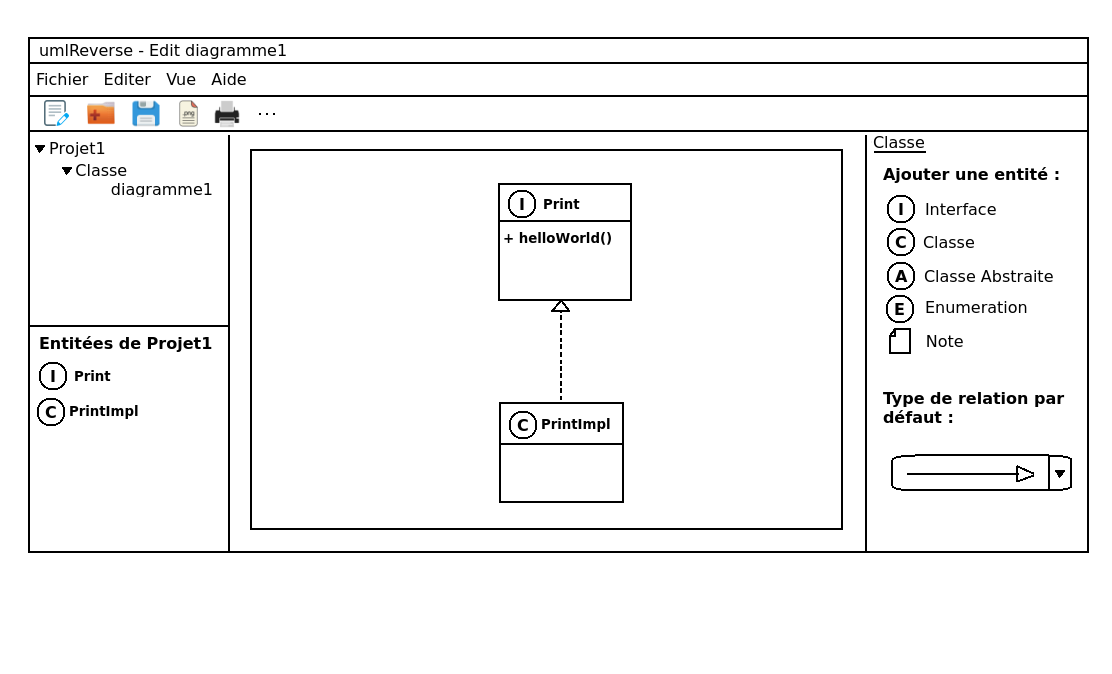
\includegraphics[width=\textwidth]{imgPDD/ihm_it2.png}
\textit{Maquette de l'interface homme-machine de l'itération 2.}
\end{center}

Disponible à la fin de la semaine 13, le but de ce livrable
sera d'implémenter l'interface homme-machine la plus fidèle à l'interface attendue à
la fin du projet. L'équipe sur l'IHM s'occupera d'étendre la vue tandis que l'équipe du 
modèle codera le modèle de diagramme de cas. 

\subsubsection{Fonctionnalités disponibles sur ce livrable}
\begin{itemize}
  \item \textbf{IHM\_10 - IHM\_20 - IHM\_30 - IHM\_50 - IHM\_60 IHM\_70 - IHM\_100} Manipuler un projet de diagramme de classe
\end{itemize}

Une définition des tâches plus précise ainsi que son attribution sera l'objet de la
préparation du sprint de l'itération 2, semaine 9/10.

\subsection{Itération 3}
\begin{center}
  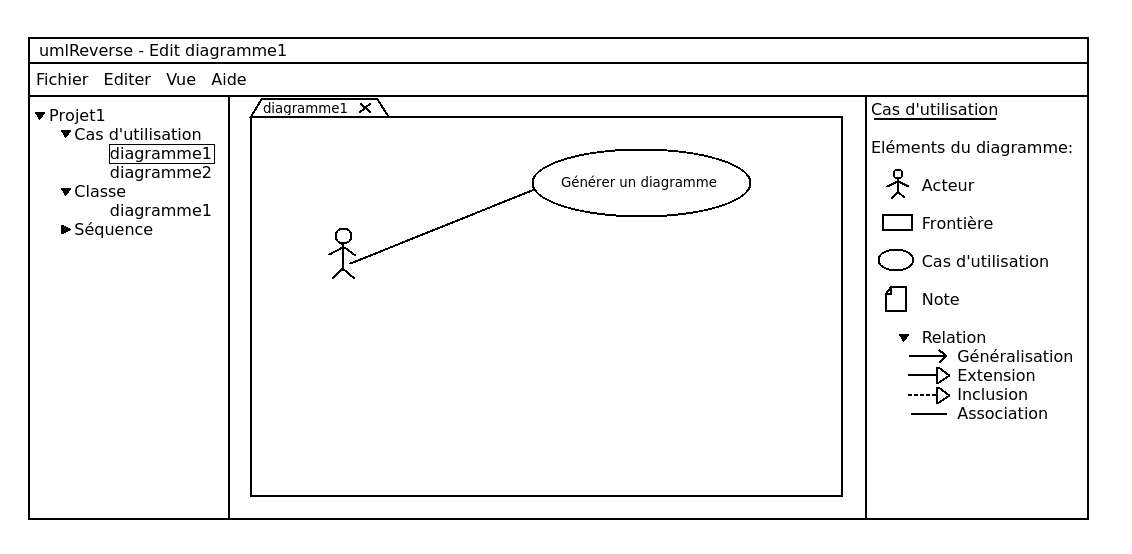
\includegraphics[width=\textwidth]{imgPDD/ihm_it3.png}
\textit{Maquette de l'interface homme-machine du livrable final.}
\end{center}

\subsubsection{Fonctionnalités disponibles sur ce livrable}
\begin{itemize}
  \item \textbf{IHM\_30 - IHM\_40 - IHM\_50 - IHM\_60 - IHM\_70 - IHM\_80 - IHM\_90 - DIA\_10} : Manipuler totalement un diagramme de cas d'utilisation
  \item \textbf{MOD\_*} : Editer un diagramme de cas d'utilisation
  \item \textbf{USE\_*} : Editer un diagramme de cas d'utilisation
\end{itemize}

Une définition des tâches plus précise ainsi que son attribution sera l'objet de la
préparation du sprint de l'itération 3, semaine 12/13.

\subsection{Evaluation de la charge de travail}

Les estimations ci-dessous sont exprimées en heures, puis en semaine/homme (s/h).
\begin{itemize}
\item \textbf{Entrée / Sortie} : Environ 20 heures, soit 3s/h.
\item \textbf{Modèle des diagrammes} : Entre 40 et 60 heures, soit de 6 à 9 s/h.
\item \textbf{IHM diagramme de classes} : Entre 30 et 50 heures, soit de 4 à 7s/h.
\item \textbf{Déplacement des entités} : Environ 10 heures, soit 1.5s/h.
\item \textbf{Gestion des relations} : Environ 15 heures, soit 2s/h.
\item \textbf{Finalisation de la partie centrale de l'IHM} : Environ 15 heures, soit 2s/h.
\item \textbf{Partie gauche de l'IHM} : Environ 40 heures, soit 6s/h.
\item \textbf{Partie droite de l'IHM} : Environ 40 heures, soit 6s/h.
\item \textbf{Fonctionnalités du menu de l'application} : Environ 35 heures, soit 5s/h.
\item \textbf{Corrections sur l'IHM} : Environ 20 à 30 heures, soit 3s/h.
Dépend des corrections demandées.
\item \textbf{IHM diagramme de cas d'utilisation} : Environ 20 à 30 heures, soit 3s/h.
\item \textbf{Finalisation du projet} : Dépend fortement de l'avancement
du projet au début de la troisième itération. Peut être estimé à environ 50 heures,
soit 8s/h.
\end{itemize}

\subsection{Disponibilités de l'équipe}
Après réunion d'équipe, chaque membre se rend disponible pour le projet environ
6 ou 7 heures par semaine. Ce temps sera réduit à environ 5 heures lors de la troisième
itération à cause des besoins de temps dans les autres matières qui vont augmenter.
Ce qui nous fait environ 200 heures de disponible lors de chacune des deux premières itérations,
et 150 heures lors de la troisième.
Un tiers de ce temps sera consacré aux activités annexes au développement de l'application,
comme les réunions client, les phases de tests fonctionnels, les réunions Scrum ou la préparation
du sprint.

\end{document}
